\documentclass[11pt,letterpaper]{article}

%----- Configuración del estilo del documento------%
\usepackage{graphicx}
\usepackage[table]{xcolor}
\usepackage[left=2cm,right=2cm,top=1.8cm,bottom=2.3cm]{geometry}
\usepackage{fancyhdr}
\usepackage{lastpage}
\usepackage[spanish]{babel}
\pagestyle{fancy}
\fancyhf{}
\rfoot{\textit{Página \thepage \hspace{1pt} de \pageref{LastPage}}}

%------ Paquetes matemáticos básicos --------%
\usepackage{amsmath, amssymb, amsthm}

%------ Texto aleatorio y listas ----- %
\usepackage{lipsum, enumitem}

\begin{document}

%------ Encabezado -------- %
\begin{center}
    \begin{minipage}{3cm}
    	\begin{center}
    		\includegraphics[height=3.4cm]{imagenes/logo_unam.png}
    	\end{center}
    \end{minipage}\hfill
    \begin{minipage}{10cm}
    	\begin{center}
    	\textbf{\large Universidad Nacional Autónoma de México}\\[0.1cm]
        \textbf{Facultad de Ciencias}\\[0.1cm]
        \textbf{Matemáticas para las Ciencias Aplicadas 2 | Grupo 7056}\\[0.1cm]
        \textbf{Tarea 1 }\\[0.1cm]
        Cisneros Álvarez Danjiro\\[0.1cm]
        Rodríguez López Luis Fernando\\[0.1cm]
        Tenorio Reyes Ihebel Luro\\[0.1cm]
        21/02/2025
    	\end{center}
    \end{minipage}\hfill
    \begin{minipage}{3cm}
    	\begin{center}
    		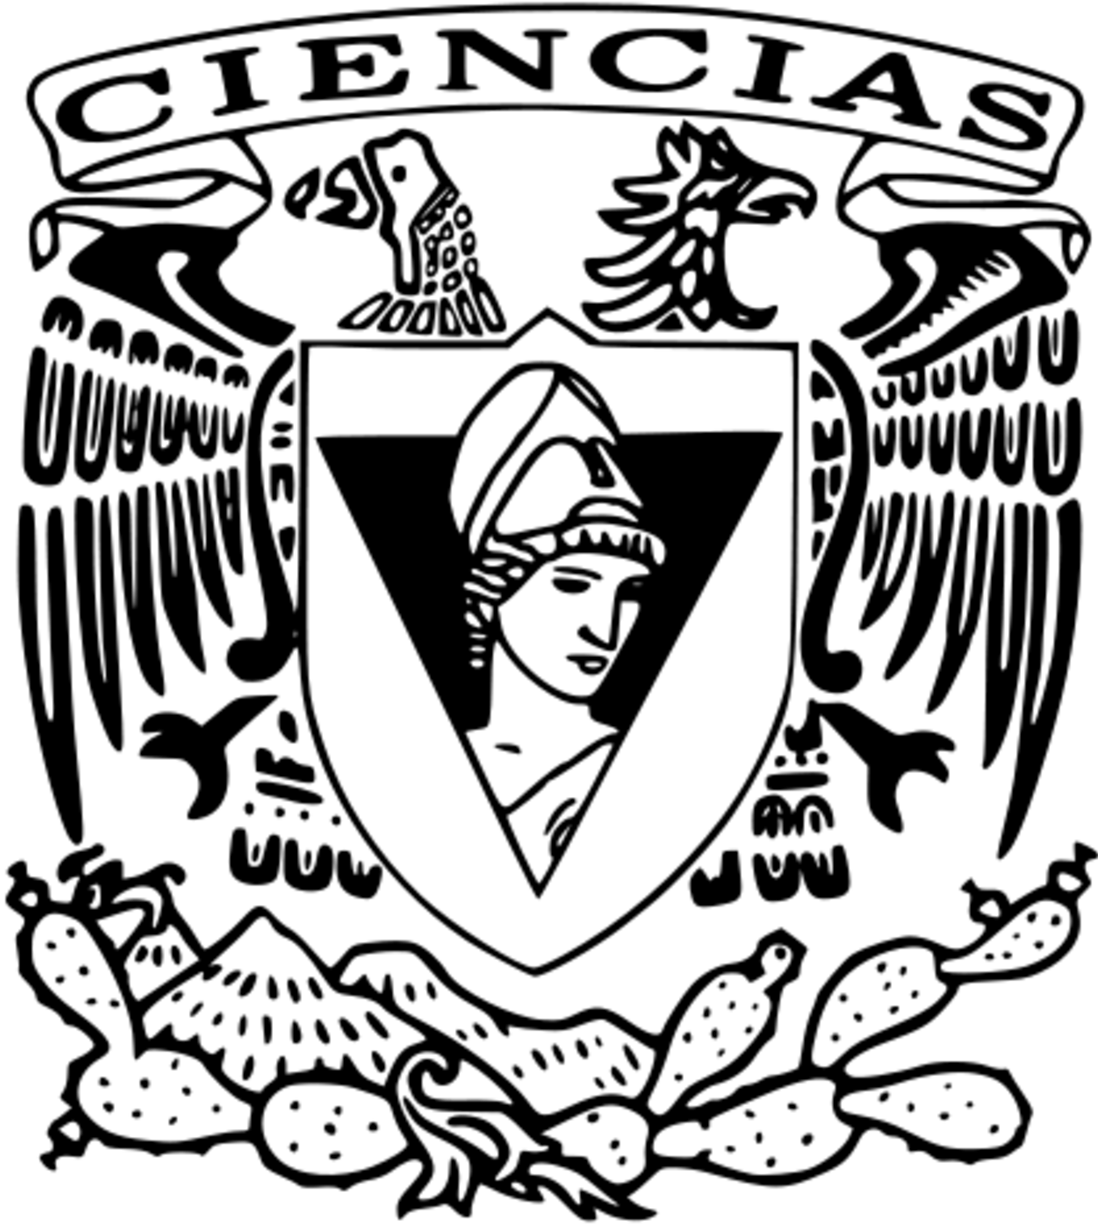
\includegraphics[height=3.4cm]{imagenes/Logo_FC.png}
    	\end{center}
    \end{minipage}
\end{center}

\noindent\rule{\linewidth}{0.4pt}

%------ Fin de encabezado -------- %

%\section*{1ra Parte}

\subparagraph{Ejercicios: Sección 11.2 Anton-Bivens-Davis (pp. 782-784).}

% ---- 01. Ejercicio 52 DANJIRO ---- %
\section{Ejercicio 52, Sección 11.2}

% ---- 02. Ejercicio 56 LUIS ---- %
\section{Ejercicio 56, Sección 11.2}
Un bloque con un peso de 100 N está suspendido por cables A y B, como se muestra en la figura adjunta.
\begin{enumerate}
    \item Utilice una herramienta gráfica para graficar las fuerzas que el bloque ejerce a lo largo de los cables A y B como funciones del ``hundimiento'' $d$.
    \item ¿El aumento del hundimiento incrementa o disminuye las fuerzas en los cables?
    \item ¿Cuánto hundimiento se requiere si los cables no pueden tolerar fuerzas superiores a 150 N?
\end{enumerate}

\begin{figure}[h]
    \centering
    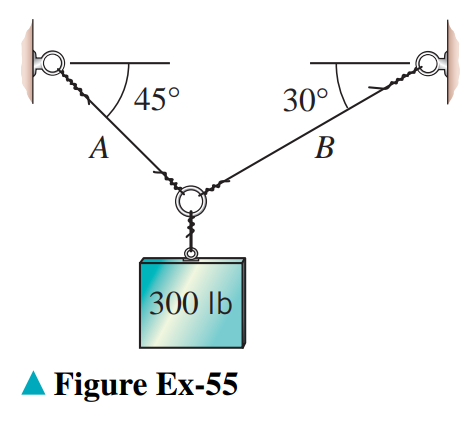
\includegraphics[width=0.2\textwidth]{imagenes/Figure_Ex-55.png}
    \hspace{5cm}
    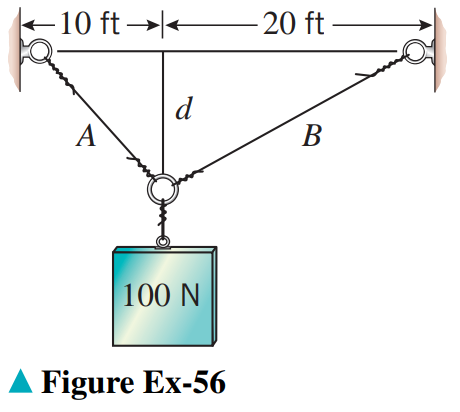
\includegraphics[width=0.2\textwidth]{imagenes/Figure_Ex-56.png}
\end{figure}


% ---- 03. Ejercicio 58 IHEBEL ---- %
\section{Ejercicio 58, Sección 11.2}


\subparagraph{Ejercicios: Sección 11.3 Anton-Bivens-Davis (pp. 792-794).}

% ---- 04. Ejercicio 19 LUIS ---- %
\section{Ejercicio 19, Sección 11.3}
La figura adjunta muestra un cubo.
\begin{enumerate}
    \item Encuentre el ángulo entre los vectores $\mathbf{d}$ y $\mathbf{u}$ al grado más cercano.
    \item Haga una conjetura sobre el ángulo entre los vectores $\mathbf{d}$ y $\mathbf{v}$, y confirme su conjetura calculando el ángulo.
\end{enumerate}

\begin{figure}[h]
    \centering
    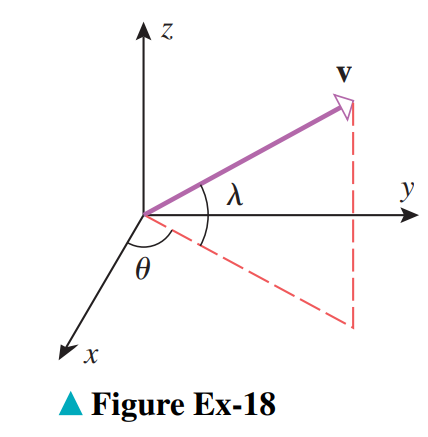
\includegraphics[width=0.2\textwidth]{imagenes/Figure_Ex-18.png}
    \hspace{5cm}
    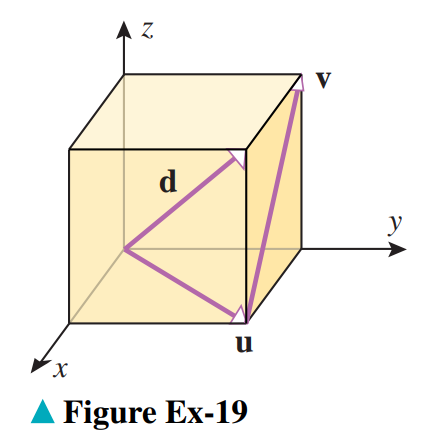
\includegraphics[width=0.2\textwidth]{imagenes/Figure_Ex-19.png}
\end{figure}


% ---- 05. Ejercicio 34 IHEBEL ---- %
\section{Ejercicio 34, Sección 11.3}

% ---- 06. Ejercicio 35 DANJIRO ---- %
\section{Ejercicio 35, Sección 11.3}

% ---- 07. Ejercicio 36 LUIS ---- %
\section{Ejercicio 36, Sección 11.3}

Suponga que el tobogán en el Ejercicio 34 tiene 4 m de largo. Estime el trabajo realizado por la gravedad si el niño se desliza desde la parte superior del tobogán hasta la parte inferior.


\subparagraph{Ejercicios: Sección 11.4 Anton-Bivens-Davis (pp. 803-805).}

% ---- 08. Ejercicio 40 IHEBEL ---- %
\section{Ejercicio 40, Sección 11.4}

% ---- 09. Ejercicio 41 DANJIRO ---- %
\section{Ejercicio 41, Sección 11.4}

% ---- 10. Ejercicio 49 POR SORTEAR ---- %
\section{Ejercicio 49, Sección 11.4}
Use un CAS para aproximar el área mínima de un triángulo si dos de sus vértices son $(2, -1, 0)$ y $(3, 2, 2)$ y su tercer vértice está en la curva $y = \ln x$ en el plano $xy$.

\end{document}